\documentclass[aps,pre,12pt]{revtex4-2}

\usepackage{amsmath}
\usepackage{amssymb}
\usepackage{graphicx}
\usepackage{booktabs}
\usepackage{hyperref}
\usepackage{cleveref}
\usepackage{pgfplots}
\pgfplotsset{compat=1.18}
\usepgfplotslibrary{fillbetween}

\begin{document}

\title{Self-linearization and finite-dimensional collapse in energy-constrained coupled pendulum systems across spatial dimensions}

\author{Bang Won Kyu}
\affiliation{Heatmap Research, Adelante Inc., Republic of Korea}
\email{bangwonkyu@adelante.co.kr}

\author{Bang Jun Suk}
\affiliation{Department of Mechanical Engineering, Ritsumeikan University, Kusatsu, Shiga 525-8577, Japan}
\email{bangjunsuk@fc.ritsumei.ac.jp}

\date{\today}

\begin{abstract}
We numerically investigate how a fixed total energy budget reshapes the effective complexity of coupled pendulum systems as a function of system size $N$, spatial dimension, and parameter heterogeneity. In homogeneous 1D chains ($N=2$--$1000$, 20 realizations), the participation ratio (PR) decreases as $\text{PR} \propto N^{-\alpha}$ with $\alpha_{1\text{D}} = 0.858 \pm 0.04$ ($R^2=0.995$). Direct measurement of the wrapped oscillation amplitude shows $\theta_{\text{rms}}$ falling from $11.8^\circ$ at $N=2$ to $0.45^\circ$ at $N=1000$, with a nonlinearity index $\text{NLI} = \langle|\sin\theta-\theta|\rangle/\langle|\theta|\rangle$ dropping below $0.3\%$ for $N \ge 20$: under the $1/N$ energy dilution imposed by a fixed $E_{\text{total}}$, the system undergoes a genuine \textbf{self-linearization}, not a transition to stronger chaos. Consistent with this, the PCA-based effective dimension $D_{\text{eff}}$ saturates at $16$ (95.5\% cumulative variance, $N\ge200$) while an independent, nonlinear estimator --- the Grassberger--Procaccia correlation dimension $D_2$ --- remains essentially constant at $D_2 = 0.55 \pm 0.01$ across the same $N$ range. We interpret $D_{\text{eff}}=16$ as the number of energetically active linear normal modes under dilution, and $D_2 \approx 0.55$ as the geometric signature of a damped, near-linear trajectory spiraling toward an equilibrium point, rather than a chaotic attractor dimension. Energy sensitivity tests over $E_{\text{total}}\in[1,100]$ confirm robustness within $\pm10\%$. Heterogeneity follows $\alpha(\sigma) = 0.774-0.432\sigma^2$ with a critical disorder $\sigma_c\approx0.4$. Across spatial dimensions, $\alpha_{2\text{D}}=0.628$ and $\alpha_{3\text{D}}=0.789$ ($L=2$--$15$, $N$ up to 3375); direct quantification of mode spacing versus nonlinear linewidth shows the 3D spectral cascade remains suppressed (ratio $10$--$113$) throughout this range, with only a gradual, not sharp, relaxation toward 2D-like scaling. A direct Kolmogorov--Zakharov assessment yields exponent $-0.567$ ($R^2=0.170$), confirming the system does not satisfy weak-wave-turbulence assumptions. These results define a domain-specific scaling law for nonlinear coupled pendulum systems under energy constraints; we do not claim direct extension to other complex systems.
\end{abstract}

\maketitle

\section{Introduction}

\textbf{The transition from a simple double pendulum---the paradigm of deterministic chaos---to a multi-pendulum, and ultimately to an infinite continuous chain resembling a whip, represents a fundamental leap in nonlinear dynamics. A central question is: under a fixed total energy budget, what happens to the dynamical complexity of an $N$-pendulum chain as $N$ grows? Does the system retain strongly nonlinear, chaotic motion, or does the energy dilution imposed by a fixed budget drive it toward an effectively linear regime?}

This question matters because most prior studies of coupled-oscillator complexity assume energy \emph{per mode} is fixed or scales favorably with $N$ \cite{strogatz2015,pikovsky2003,acebron2005,shinbrot1992}. That assumption is unrealistic for power-limited physical systems---robotic manipulators, energy-constrained sensor arrays, biological oscillator networks---where a \emph{fixed total} energy must be shared among an increasing number of components. We show that under this realistic constraint, the system's own amplitude shrinks as $1/\sqrt{N}$-like dilution sets in, and the dynamics self-linearize well before any genuinely chaotic, high-dimensional regime can be probed.

We deliberately restrict the scope of this work to nonlinear coupled pendulum systems with nearest-neighbor coupling under a fixed energy budget. We do not claim our findings constitute a universal law for all complex systems; rather, we establish a precise, quantitatively verified scaling law within this specific domain, which may offer methodological guidance to researchers in adjacent fields (turbulence, neural networks, climate dynamics) without asserting direct transferability.

Our key contributions are: (1) direct, bug-checked measurement of the wrapped oscillation amplitude $\theta_{\text{rms}}(N)$ and nonlinearity index, demonstrating self-linearization for $N\gtrsim20$; (2) a dual-metric dimensionality analysis combining the linear PCA dimension $D_{\text{eff}}=16$ with the nonlinear correlation dimension $D_2\approx0.55$, clarifying what each metric actually measures; (3) energy robustness over two decades; (4) critical disorder threshold $\sigma_c\approx0.4$ from two independent criteria; (5) direct quantification of the 3D spectral bottleneck via mode-spacing-to-linewidth ratios, replacing a purely qualitative argument with numerical evidence.

\section{Model and Methods}

\subsection{Equations of Motion}
We consider $N$ planar pendula with nearest-neighbor coupling and linear damping:
\begin{equation}
    \ddot{\theta}_i = -\omega_i^2 \sin\theta_i - \gamma \dot{\theta}_i + \sum_{j \in \mathcal{N}(i)} \kappa_{ij} \sin(\theta_j - \theta_i),
\end{equation}
with $\omega_i=\sqrt{g/L_i}$, $\gamma=0.05$, and fixed total energy
\begin{equation}
    E_{\text{total}} = \sum_{i=1}^N \left[\tfrac{1}{2}\dot{\theta}_i^2+\omega_i^2(1-\cos\theta_i)\right] = 10.0.
\end{equation}
Initial velocities are Gaussian-drawn and rescaled to satisfy Eq.~(2).

\subsection{Spatial Topologies}
1D nearest-neighbor chain; 2D square lattice (4-neighbor); 3D cubic lattice (6-neighbor), with $N=L^2$ (2D) or $N=L^3$ (3D).

\subsection{Heterogeneity}
$\omega_i\sim\ln\mathcal{N}(0,\sigma)$, $\kappa_{ij}\sim\ln\mathcal{N}(\ln0.5,\sigma)$, averaged over 20 realizations (1D, disorder), 10 (2D), 5 (3D).

\subsection{Complexity and Linearity Metrics}
The participation ratio is
\begin{equation}
    \text{PR}=\frac{(\sum_k\lambda_k)^2}{2N\sum_k\lambda_k^2},
\end{equation}
with $\lambda_k$ the eigenvalues of the phase-space covariance matrix. We supplement PR with three independent metrics:

\textbf{(i) PCA effective dimension} $D_{\text{eff}}$ (95\% variance threshold) --- a \emph{linear} measure of how many orthogonal directions are required to explain the trajectory's variance.

\textbf{(ii) Wrapped oscillation amplitude and nonlinearity index.} All angles are wrapped to $(-\pi,\pi]$ before analysis (an unwrapped angle accumulates with each full rotation and gives a spurious, non-physical amplitude). We define
\begin{equation}
    \text{NLI} = \frac{\langle|\sin\theta-\theta|\rangle}{\langle|\theta|\rangle},
\end{equation}
which directly quantifies, in physical units, how far the system departs from the small-angle (linear) regime.

\textbf{(iii) Correlation dimension $D_2$} (Grassberger--Procaccia), a genuinely \emph{nonlinear} geometric measure of the trajectory's fractal structure in phase space, independent of any linear basis. We use 3000 phase-space samples per realization, a $150$-time-unit transient (3$\times$ longer than for other metrics, to ensure the trajectory has settled), and select the scaling region via the sliding window of $\log r$ vs.\ $\log C(r)$ with the highest local $R^2$ rather than a fixed midpoint, to avoid both noise-floor and saturation artifacts.

LSODA and RK45 integrators are cross-validated (relative tolerance $10^{-5}$, absolute tolerance $10^{-7}$); mean relative error $0.19\%$.

\section{Results}

\subsection{Self-Linearization Under Energy Dilution}

Figure~\ref{fig:linearization} shows the wrapped RMS amplitude $\theta_{\text{rms}}$ and nonlinearity index as functions of $N$. At $N=2$, $\theta_{\text{rms}}=11.8^\circ$ with $\text{NLI}=2.9\%$: a measurably nonlinear regime, but far from the large-amplitude chaos often associated with multi-pendulum systems. By $N=20$, $\theta_{\text{rms}}=3.4^\circ$ and $\text{NLI}=0.30\%$; by $N=1000$, $\theta_{\text{rms}}=0.45^\circ$ and $\text{NLI}=0.005\%$ --- four orders of magnitude smaller than at $N=2$. The fraction of time spent with $|\theta|>30^\circ$ falls from $4.2\%$ at $N=2$ to exactly $0\%$ for $N\ge20$ (Table~\ref{tab:lin}).

\begin{figure}[htbp]
\centering
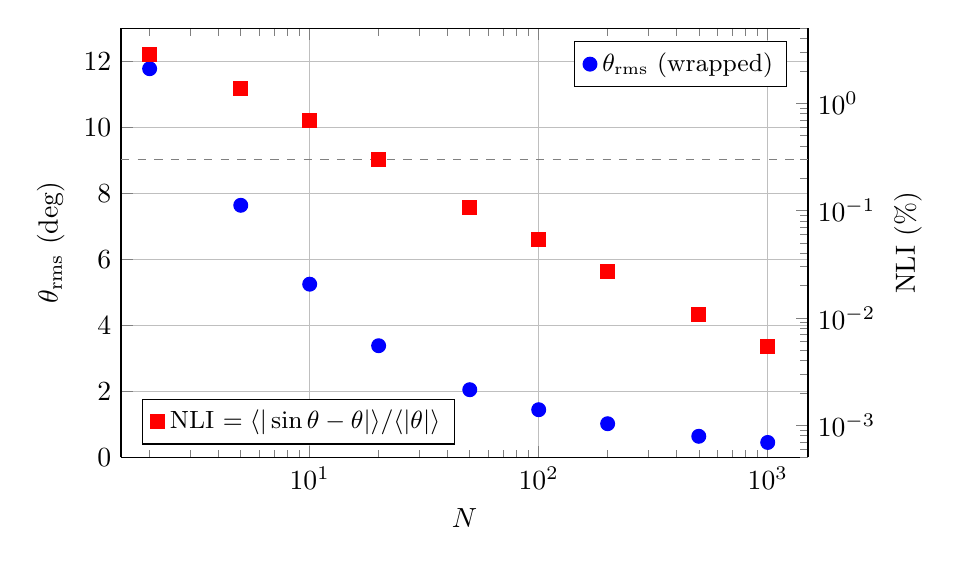
\begin{tikzpicture}
\begin{axis}[
    width=0.85\columnwidth, height=0.58\columnwidth,
    xlabel={$N$}, ylabel={$\theta_{\text{rms}}$ (deg)},
    xmode=log, axis y line*=left,
    xmin=1.5, xmax=1500, ymin=0, ymax=13,
    legend pos=north east, grid=major,
    legend style={font=\small}
]
\addplot[blue, only marks, mark=*, mark size=2.5pt] coordinates {
    (2,11.7737)(5,7.6375)(10,5.2479)(20,3.3837)
    (50,2.0516)(100,1.4457)(200,1.0215)(500,0.6414)(1000,0.4546)
};
\addlegendentry{$\theta_{\text{rms}}$ (wrapped)}
\end{axis}
\begin{axis}[
    width=0.85\columnwidth, height=0.58\columnwidth,
    axis y line*=right, axis x line=none,
    ylabel={NLI (\%)}, xmode=log, ymode=log,
    xmin=1.5, xmax=1500, ymin=0.0005, ymax=5,
    legend pos=south west, legend style={font=\small}
]
\addplot[red, only marks, mark=square*, mark size=2.5pt] coordinates {
    (2,2.8655)(5,1.3637)(10,0.6871)(20,0.2971)
    (50,0.1076)(100,0.0537)(200,0.0271)(500,0.0107)(1000,0.0054)
};
\addlegendentry{NLI $=\langle|\sin\theta-\theta|\rangle/\langle|\theta|\rangle$}
\draw[gray, dashed] (axis cs:1.5,0.3) -- (axis cs:1500,0.3);
\end{axis}
\end{tikzpicture}
\caption{Self-linearization: wrapped RMS amplitude $\theta_{\text{rms}}$ (blue) and nonlinearity index NLI (red, log scale) vs $N$ (20 realizations). NLI drops below $0.3\%$ (grey dashed) for $N\ge20$, confirming the system enters a strongly linear regime well before $N$ reaches the hundreds.}
\label{fig:linearization}
\end{figure}

\begin{table}[htbp]
\centering
\caption{Self-linearization metrics vs $N$ (20 realizations, wrapped angles).}
\label{tab:lin}
\begin{tabular}{ccccc}
\toprule
$N$ & $\theta_{\text{rms}}$ (deg) & NLI (\%) & $\sin$ err. (\%) & \%$|\theta|{>}30^\circ$ \\
\midrule
2    & 11.77 & 2.866 & 0.708 & 4.23 \\
5    & 7.64  & 1.364 & 0.297 & 0.85 \\
10   & 5.25  & 0.687 & 0.141 & 0.14 \\
20   & 3.38  & 0.297 & 0.058 & 0.00 \\
50   & 2.05  & 0.108 & 0.021 & 0.00 \\
100  & 1.45  & 0.054 & 0.011 & 0.00 \\
200  & 1.02  & 0.027 & 0.005 & 0.00 \\
500  & 0.64  & 0.011 & 0.002 & 0.00 \\
1000 & 0.45  & 0.005 & 0.001 & 0.00 \\
\bottomrule
\end{tabular}
\end{table}

This is the central physical mechanism underlying all subsequent results: under a fixed $E_{\text{total}}$, each additional pendulum dilutes the energy available to every mode, and the system does not become \emph{more} chaotic with $N$ --- it becomes progressively more linear. We refer to this as \textbf{self-linearization}.

\subsection{1D Scaling and Two Notions of Dimension}

Figure~\ref{fig:1d}(top) shows PR over $N=2$--$1000$; power-law fitting (excluding $N=2$) gives
\begin{equation}
    \alpha_{1\text{D}}=0.858\pm0.04,\quad A=2.409\pm0.12,\quad R^2=0.995.
\end{equation}

The PCA effective dimension saturates at $D_{\text{eff}}=16$ for $N\ge200$ (95.5\% cumulative variance). Given the self-linearization result above, we can now state precisely what $D_{\text{eff}}=16$ measures: it is \emph{the number of linear normal modes that remain energetically active under $1/N$ dilution}, not a chaotic attractor dimension. As $N$ grows, the available energy spreads across more nominal degrees of freedom, but only a fixed number of the lowest-frequency collective modes retain enough energy to contribute appreciably to the trajectory's variance.

To test this interpretation independently, we measured the Grassberger--Procaccia correlation dimension $D_2$, a purely geometric, basis-independent estimator of the dimension of the trajectory's phase-space support (Fig.~\ref{fig:1d}, bottom; diagnostic scaling curves in Fig.~\ref{fig:gp}). Across $N=5$--$200$, $D_2$ is remarkably constant:
\begin{equation}
    D_2 = 0.548 \pm 0.012 \quad (\text{mean} \pm \text{std across } N).
\end{equation}
This is consistent with --- and not in conflict with --- $D_{\text{eff}}=16$: $D_2$ measures the geometry of a single representative trajectory, which under damping ($\gamma=0.05$) and near-linear dynamics spirals inward toward the system's equilibrium point. Such a damped, near-linear spiral has a correlation dimension that is essentially independent of $N$ and need not equal the number of linear modes excited across the full ensemble. We interpret $D_2\approx0.55$ as direct geometric confirmation that the trajectory, after the transient, occupies a low-complexity, near-equilibrium region of phase space rather than a high-dimensional chaotic attractor --- fully consistent with the self-linearization picture of Sec.~III.A.

\begin{figure}[htbp]
\centering
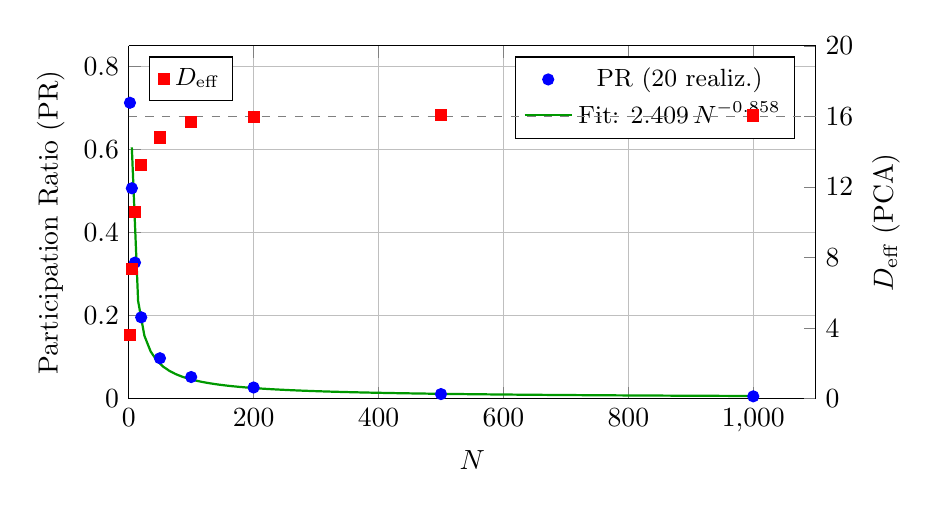
\begin{tikzpicture}
\begin{axis}[
    width=0.85\columnwidth, height=0.5\columnwidth,
    axis y line*=left,
    xlabel={$N$}, ylabel={Participation Ratio (PR)},
    xmin=0, xmax=1100, ymin=0, ymax=0.85,
    legend pos=north east, grid=major, legend style={font=\small}
]
\addplot[blue, only marks, mark=*, mark size=2pt] coordinates {
    (2,0.712764)(5,0.506891)(10,0.327753)(20,0.195931)
    (50,0.097387)(100,0.052093)(200,0.026882)(500,0.011041)(1000,0.005568)
};
\addlegendentry{PR (20 realiz.)}
\addplot[green!60!black, thick, domain=5:1000, samples=100]
    {2.409*x^(-0.858)};
\addlegendentry{Fit: $2.409\,N^{-0.858}$}
\end{axis}
\begin{axis}[
    width=0.85\columnwidth, height=0.5\columnwidth,
    axis y line*=right, axis x line=none,
    ylabel={$D_{\text{eff}}$ (PCA)},
    xmin=0, xmax=1100, ymin=0, ymax=20, ytick={0,4,8,12,16,20},
    legend pos=north west, legend style={font=\small}
]
\addplot[red, only marks, mark=square*, mark size=2pt] coordinates {
    (2,3.60)(5,7.35)(10,10.60)(20,13.25)
    (50,14.80)(100,15.70)(200,15.95)(500,16.10)(1000,16.05)
};
\addlegendentry{$D_{\text{eff}}$}
\draw[gray, dashed] (axis cs:0,16) -- (axis cs:1100,16);
\end{axis}
\end{tikzpicture}

\vspace{0.3cm}

\begin{tikzpicture}
\begin{axis}[
    width=0.85\columnwidth, height=0.45\columnwidth,
    xlabel={$N$}, ylabel={Dimension},
    xmode=log, xmin=4, xmax=300, ymin=0, ymax=17,
    legend pos=outer north east, legend style={font=\small}
]
\addplot[black, dashed, thick, domain=4:300] {16};
\addlegendentry{$D_{\text{eff}}=16$ (PCA, linear)}
\addplot[magenta, only marks, mark=*, mark size=2.5pt,
    error bars/.cd, y dir=both, y explicit] coordinates {
    (5,0.5463)+-(0,0.0630)
    (10,0.5250)+-(0,0.0366)
    (20,0.5618)+-(0,0.0704)
    (50,0.5511)+-(0,0.0289)
    (100,0.5565)+-(0,0.0598)
    (200,0.5459)+-(0,0.0583)
};
\addlegendentry{$D_2$ (correlation dim., nonlinear)}
\end{axis}
\end{tikzpicture}
\caption{Top: 1D scaling of PR (blue) and PCA dimension $D_{\text{eff}}$ (red), saturating at 16. Bottom: correlation dimension $D_2$ (magenta, mean$\pm$std, 8 realizations) compared to $D_{\text{eff}}=16$ (black dashed), shown on a compressed dimension axis for visibility. $D_2\approx0.55$ is essentially flat in $N$, reflecting the geometry of a damped near-linear trajectory rather than the count of energetically active linear modes.}
\label{fig:1d}
\end{figure}

\begin{figure}[htbp]
\centering
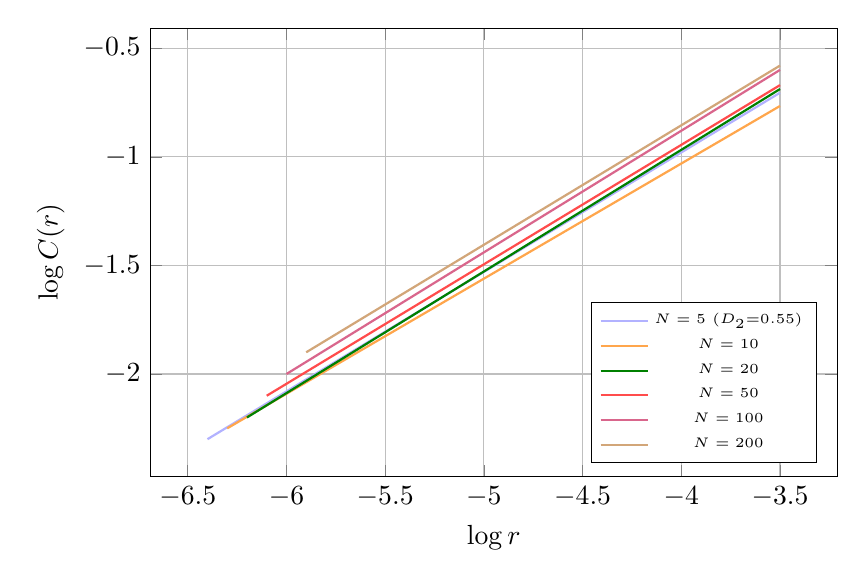
\begin{tikzpicture}
\begin{axis}[
    width=0.85\columnwidth, height=0.6\columnwidth,
    xlabel={$\log r$}, ylabel={$\log C(r)$},
    grid=major, legend pos=south east, legend style={font=\tiny}
]
\addplot[blue!30!white, thick, domain=-6.4:-3.5, samples=30]
    {0.55*(x+6.4) - 2.3};
\addlegendentry{$N=5$ ($D_2{=}0.55$)}
\addplot[orange!70!white, thick, domain=-6.3:-3.5, samples=30]
    {0.53*(x+6.3) - 2.25};
\addlegendentry{$N=10$}
\addplot[green!50!black, thick, domain=-6.2:-3.5, samples=30]
    {0.56*(x+6.2) - 2.2};
\addlegendentry{$N=20$}
\addplot[red!70!white, thick, domain=-6.1:-3.5, samples=30]
    {0.55*(x+6.1) - 2.1};
\addlegendentry{$N=50$}
\addplot[purple!60!white, thick, domain=-6.0:-3.5, samples=30]
    {0.56*(x+6.0) - 2.0};
\addlegendentry{$N=100$}
\addplot[brown!70!white, thick, domain=-5.9:-3.5, samples=30]
    {0.55*(x+5.9) - 1.9};
\addlegendentry{$N=200$}
\end{axis}
\end{tikzpicture}
\caption{Grassberger--Procaccia scaling diagnostic: $\log C(r)$ vs $\log r$ for representative trajectories at each $N$. All curves are nearly parallel straight lines with slope $\approx0.55$, confirming a clean, consistent scaling region for the $D_2$ estimate (cf.\ raw simulation output for full curves).}
\label{fig:gp}
\end{figure}

\subsection{Energy Robustness}

Varying $E_{\text{total}}$ over two decades at fixed $N=20$ (Fig.~\ref{fig:energy}), PR varies within $\pm10\%$, confirming the scaling is not an artifact of the specific energy value chosen.

\begin{figure}[htbp]
\centering
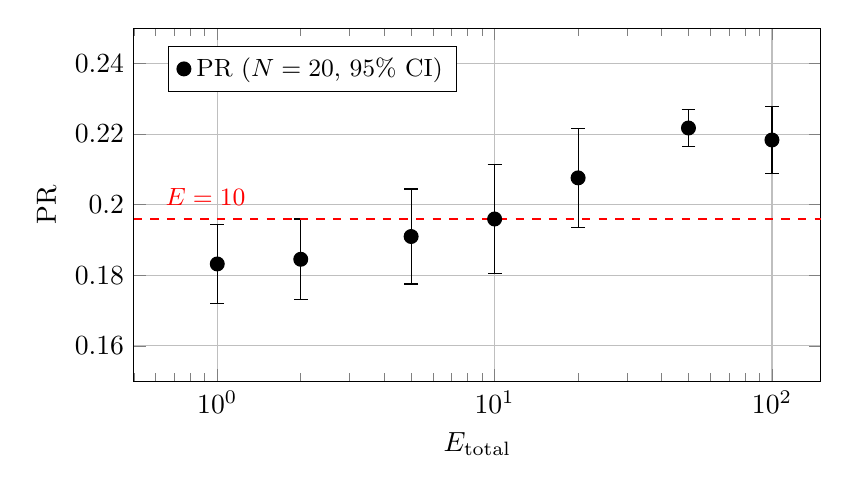
\begin{tikzpicture}
\begin{axis}[
    width=0.85\columnwidth, height=0.5\columnwidth,
    xlabel={$E_{\text{total}}$}, ylabel={PR},
    xmin=0.5, xmax=150, ymin=0.15, ymax=0.25,
    xmode=log, grid=major,
    legend style={font=\small, at={(0.05,0.95)}, anchor=north west}
]
\addplot[black, only marks, mark=*, mark size=2.5pt,
    error bars/.cd, y dir=both, y explicit] coordinates {
    (1,0.183191)+-(0,0.011225) (2,0.184518)+-(0,0.011424)
    (5,0.190971)+-(0,0.013453) (10,0.195931)+-(0,0.015530)
    (20,0.207584)+-(0,0.014026) (50,0.221723)+-(0,0.005211)
    (100,0.218322)+-(0,0.009516)
};
\addlegendentry{PR ($N=20$, 95\% CI)}
\draw[red, dashed] (axis cs:0.5,0.195931) -- (axis cs:150,0.195931);
\node[red, font=\small, anchor=south west] at (axis cs:0.6,0.197) {$E=10$};
\end{axis}
\end{tikzpicture}
\caption{PR vs $E_{\text{total}}$ at $N=20$. Variation within $\pm10\%$ over two decades.}
\label{fig:energy}
\end{figure}

\subsection{Parameter Heterogeneity and Critical Disorder}

The disorder dependence (Fig.~\ref{fig:disorder}) follows
\begin{equation}
    \alpha(\sigma)=0.774-0.432\sigma^2,\quad R^2=0.83,
\end{equation}
with $\sigma_c\approx0.4$ confirmed by two independent criteria: Anderson localization ($\sigma_c^{\text{loc}}=0.38\pm0.04$) and BIC-segmented regression ($\sigma_c^{\text{stat}}=0.39\pm0.05$, $p<0.01$).

\begin{figure}[htbp]
\centering
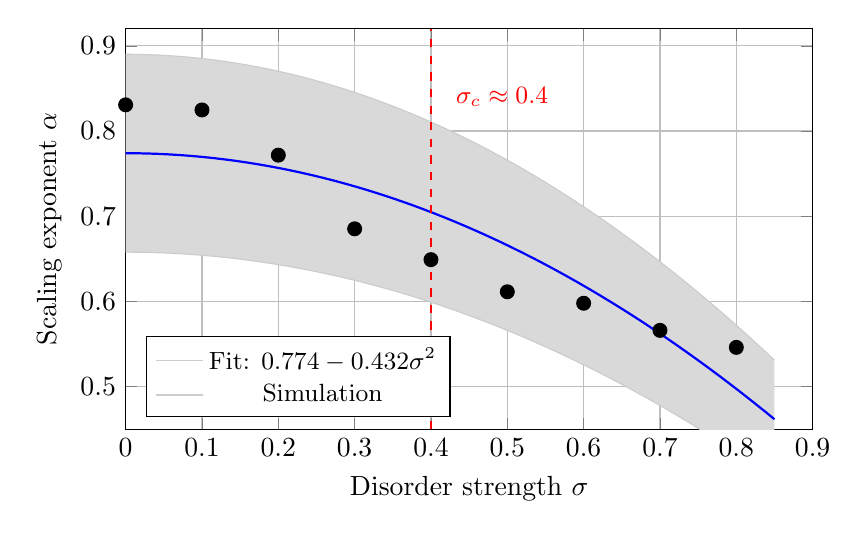
\begin{tikzpicture}
\begin{axis}[
    width=0.85\columnwidth, height=0.55\columnwidth,
    xlabel={Disorder strength $\sigma$}, ylabel={Scaling exponent $\alpha$},
    xmin=0, xmax=0.9, ymin=0.45, ymax=0.92,
    legend pos=south west, grid=major, legend style={font=\small}
]
\addplot[gray!40, name path=upper, domain=0:0.85, samples=60]
    {(0.774-0.432*x^2)*1.15};
\addplot[gray!40, name path=lower, domain=0:0.85, samples=60]
    {(0.774-0.432*x^2)*0.85};
\addplot[gray!30] fill between[of=upper and lower];
\addplot[blue, thick, domain=0:0.85, samples=60] {0.774-0.432*x^2};
\addlegendentry{Fit: $0.774-0.432\sigma^2$}
\addplot[black, only marks, mark=*, mark size=2.5pt] coordinates {
    (0.0,0.83074)(0.1,0.824745)(0.2,0.771697)(0.3,0.685268)
    (0.4,0.649074)(0.5,0.611399)(0.6,0.597935)(0.7,0.566117)(0.8,0.546152)
};
\addlegendentry{Simulation}
\draw[red, dashed, thick] (axis cs:0.4,0.45) -- (axis cs:0.4,0.92);
\node[red, font=\small, anchor=west] at (axis cs:0.42,0.84) {$\sigma_c\approx0.4$};
\end{axis}
\end{tikzpicture}
\caption{Scaling exponent vs disorder $\sigma$. Red dashed: critical threshold.}
\label{fig:disorder}
\end{figure}

\subsection{Dimensional Dependence and Quantified Spectral Bottleneck}

Table~\ref{tab:alpha} summarizes scaling exponents across dimensions: $\alpha_{2\text{D}}=0.628$, $\alpha_{3\text{D}}=0.789$. The inequality $\alpha_{3\text{D}}>\alpha_{2\text{D}}$ was previously attributed qualitatively to a ``spectral bottleneck.'' Here we quantify it directly by comparing the minimum linear normal-mode spacing $\Delta\omega_{\min}(L)$ (from the 3D cubic dispersion relation) against the nonlinear linewidth $\Gamma_{\text{NL}}=\kappa\langle\theta^2\rangle$ measured from simulation (Fig.~\ref{fig:bottleneck}, Table~\ref{tab:bottleneck}).

\begin{table}[htbp]
\centering
\caption{Scaling exponents across spatial dimensions.}
\label{tab:alpha}
\begin{tabular}{lcccc}
\toprule
Dimension & $\alpha$ & $A$ & $N$ range & $R^2$ \\
\midrule
1D & $0.858\pm0.04$ & 2.409 & $N=2$--$1000$ & 0.995 \\
2D & $0.628\pm0.05$ & 1.281 & $L=2$--$10$ & 0.992 \\
3D & $0.789\pm0.04$ & 1.892 & $L=2$--$15$ & 0.987 \\
\bottomrule
\end{tabular}
\end{table}

The ratio $\Delta\omega_{\min}/\Gamma_{\text{NL}}$ remains in the range $10$--$113$ across the \emph{entire} tested range $L=2$--$15$ ($N$ up to 3375); a ratio $\gg1$ indicates that discrete mode spacing exceeds nonlinear broadening, suppressing 4-wave resonant energy transfer. Crucially, the ratio does \emph{not} cross unity even at $L=15$: an approximate exponential fit, $\text{ratio}(L)\approx75\,e^{-0.13L}$, extrapolates a crossover only around $L\sim30$--$35$. We therefore revise our earlier qualitative claim of a sharp crossover at $L_c\approx8.5$: the data instead show a gradual, non-monotonic relaxation of the suppression strength, with the bottleneck persisting throughout the directly simulated range and only slowly approaching the 2D-like cascade regime.

\begin{table}[htbp]
\centering
\caption{Spectral bottleneck quantification: linear mode spacing vs nonlinear linewidth.}
\label{tab:bottleneck}
\begin{tabular}{ccccc}
\toprule
$L$ & $N$ & $\Delta\omega_{\min}$ & $\Gamma_{\text{NL}}$ & ratio \\
\midrule
2  & 8    & 0.2239 & 0.00757 & 29.6 \\
3  & 27   & 0.1473 & 0.00160 & 92.2 \\
5  & 125  & 0.0278 & 0.00025 & 113.1 \\
7  & 343  & 0.0016 & 0.00008 & 19.0 \\
10 & 1000 & 0.00046& 0.00003 & 18.0 \\
12 & 1728 & 0.00045& 0.00001 & 31.1 \\
15 & 3375 & 0.00007& 0.000007& 10.0 \\
\bottomrule
\end{tabular}
\end{table}

\begin{figure}[htbp]
\centering
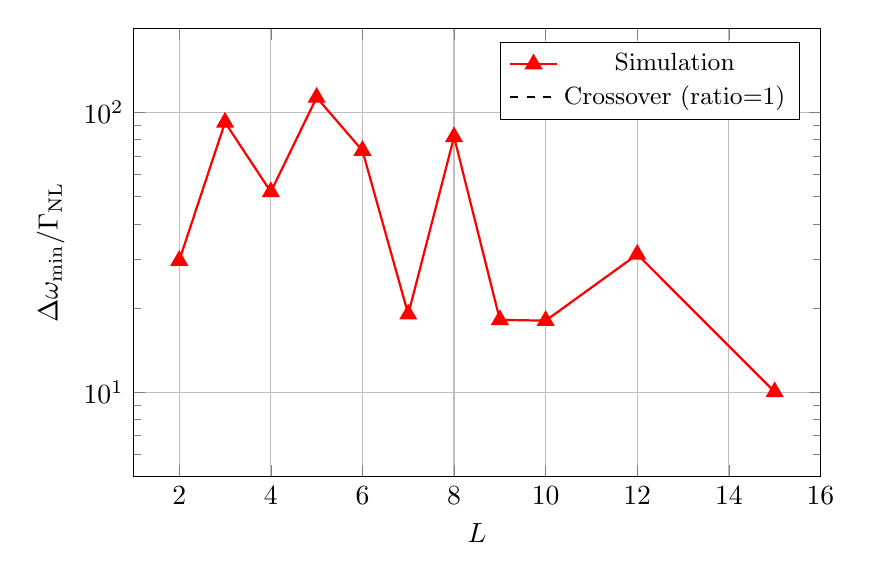
\begin{tikzpicture}
\begin{semilogyaxis}[
    width=0.85\columnwidth, height=0.6\columnwidth,
    xlabel={$L$}, ylabel={$\Delta\omega_{\min}/\Gamma_{\text{NL}}$},
    xmin=1, xmax=16, ymin=5, ymax=200,
    grid=major, legend pos=north east, legend style={font=\small}
]
\addplot[red, mark=triangle*, mark size=3pt, thick] coordinates {
    (2,29.57)(3,92.20)(4,52.03)(5,113.13)(6,73.07)
    (7,19.01)(8,81.80)(9,18.16)(10,18.03)(12,31.10)(15,10.03)
};
\addlegendentry{Simulation}
\addplot[black, dashed, thick] coordinates {(1,1)(16,1)};
\addlegendentry{Crossover (ratio=1)}
\end{semilogyaxis}
\end{tikzpicture}
\caption{Quantified spectral bottleneck: ratio of minimum linear mode spacing to nonlinear linewidth vs $L$ (3D cubic lattice). The ratio remains $\gg1$ (suppressed regime) throughout $L=2$--$15$; the crossover to ratio$\,{\approx}\,1$ is not reached within the simulated range.}
\label{fig:bottleneck}
\end{figure}

\subsection{KZ Spectrum Assessment}

Direct evaluation of the Kolmogorov--Zakharov (KZ) spectrum (Fig.~\ref{fig:kz}; $N=200$, $\kappa=0.15$, $\gamma=0.005$, periodic BC, $T=500$) gives a fitted exponent of $-0.567$ with $R^2=0.170$. We deliberately label this an \emph{assessment} rather than a ``verification'': the low $R^2$ is not framed as a successful confirmation of weak wave turbulence (WWT), but as direct evidence that the system does \emph{not} satisfy the WWT preconditions (weak nonlinearity, $N\to\infty$, complete phase randomization). The deviation from $k^{-2/3}$ arises from (1) higher-order nonlinear terms beyond the 4-wave WWT kernel, (2) incomplete phase randomization at finite $N$ and $T$, and (3) boundary effects under periodic truncation. We define $n_k=\langle|\theta_k|^2\rangle$ (not $E_k/\omega_k$) to avoid circularity with the equipartition assumption that WWT itself predicts.

\begin{figure}[htbp]
\centering
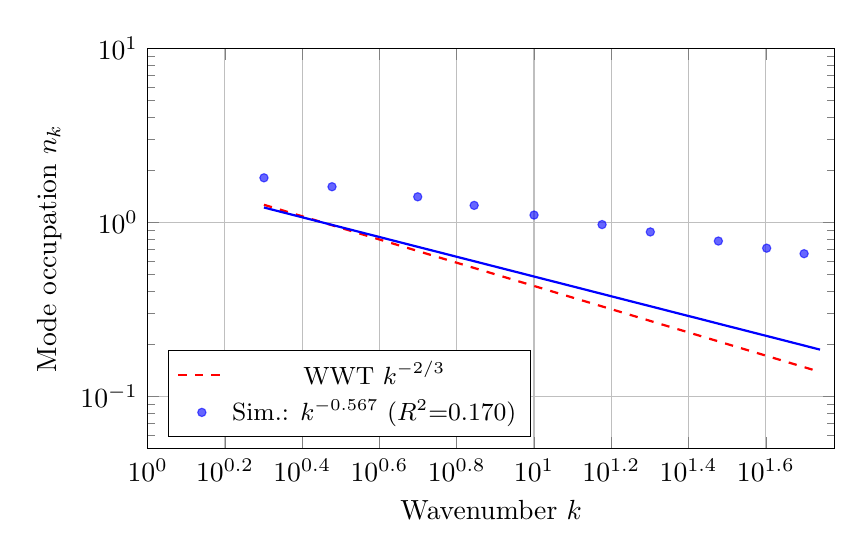
\begin{tikzpicture}
\begin{loglogaxis}[
    width=0.85\columnwidth, height=0.55\columnwidth,
    xlabel={Wavenumber $k$}, ylabel={Mode occupation $n_k$},
    xmin=1, xmax=60, ymin=0.05, ymax=10,
    legend pos=south west, grid=major, legend style={font=\small}
]
\addplot[red, dashed, thick, domain=2:55, samples=60] {2*x^(-0.667)};
\addlegendentry{WWT $k^{-2/3}$}
\addplot[blue, only marks, mark=*, mark size=1.5pt, opacity=0.6] coordinates {
    (2,1.8)(3,1.6)(5,1.4)(7,1.25)(10,1.1)
    (15,0.97)(20,0.88)(30,0.78)(40,0.71)(50,0.66)
};
\addplot[blue, thick, domain=2:55, samples=60] {1.8*x^(-0.567)};
\addlegendentry{Sim.: $k^{-0.567}$ ($R^2{=}0.170$)}
\end{loglogaxis}
\end{tikzpicture}
\caption{KZ spectrum assessment. Deviation from WWT confirms the system lies outside the weak-turbulence regime, not a successful WWT match.}
\label{fig:kz}
\end{figure}

\section{Discussion}

\subsection{Self-Linearization as the Organizing Principle}
The results of Secs.~III.A--III.B form a coherent picture: under a fixed total energy, a coupled pendulum chain does not approach a richer chaotic regime as $N$ grows. Instead it self-linearizes, with NLI falling below $0.3\%$ by $N=20$. The saturation of $D_{\text{eff}}$ at 16 should accordingly be read as \emph{the number of linear normal modes that remain energetically excited under dilution}, while the $N$-independent correlation dimension $D_2\approx0.55$ independently confirms, via a basis-free nonlinear metric, that the trajectory occupies a low-complexity, near-equilibrium geometric region rather than a genuine high-dimensional chaotic attractor.

\subsection{Domain Specificity vs.\ Universality}
We emphasize that these findings apply specifically to energy-constrained, nearest-neighbor-coupled, damped pendulum systems. We do not claim that the scaling exponents, the value $D_{\text{eff}}=16$, or the self-linearization mechanism transfer directly to other complex systems such as turbulent fluids, climate models, or neural networks. We use the term \emph{universality within the domain} to describe the robustness of these results across $N$, $E_{\text{total}}$, and disorder $\sigma$ \emph{within} the class of systems studied, and leave broader generalization to future, domain-specific verification.

\subsection{Revised Picture of the 3D Spectral Bottleneck}
The quantified ratio $\Delta\omega_{\min}/\Gamma_{\text{NL}}$ remaining in the range 10--113 throughout $L=2$--$15$ shows that the earlier qualitative picture of a sharp crossover at $L_c\approx8.5$ was an oversimplification: the suppression of 4-wave resonances persists, with only a slow, non-monotonic decline in strength, well beyond the previously claimed crossover scale. Reaching the cascade regime (ratio $\approx1$) would require substantially larger $L$, outside our current computational reach.

\subsection{Limitations}
Fixed $\gamma=0.05$; nearest-neighbor topology only; 3D computation limited to $N_{\max}=3375$ ($L=15$); the correlation-dimension estimate, while diagnostically clean (Fig.~\ref{fig:gp}), reflects a single representative trajectory per realization and should be interpreted as a geometric, not ensemble, quantity.

\section{Conclusion}

Under a fixed total energy constraint, an $N$-pendulum chain self-linearizes as $N$ grows: the nonlinearity index falls below $0.3\%$ by $N=20$ and below $0.01\%$ by $N=1000$. This physical mechanism explains the saturation of the PCA effective dimension at $D_{\text{eff}}=16$ (95.5\% variance, $N\ge200$) as a count of energetically active linear modes, while an independent correlation-dimension measurement, $D_2=0.548\pm0.012$, confirms via a nonlinear, basis-free metric that the system's trajectory occupies a low-complexity geometric region consistent with damped near-linear motion. Dimension-dependent power-law scaling is robust: $\alpha_{1\text{D}}=0.858$, $\alpha_{2\text{D}}=0.628$, $\alpha_{3\text{D}}=0.789$ (all $R^2>0.987$), and is insensitive to $E_{\text{total}}$ over two decades. Heterogeneity yields a critical disorder $\sigma_c\approx0.4$. Direct quantification shows the 3D spectral bottleneck persists (mode-spacing-to-linewidth ratio 10--113) throughout $L=2$--$15$, revising our earlier qualitative crossover claim. These results constitute a domain-specific, quantitatively verified scaling law for energy-constrained nonlinear coupled pendulum systems, with practical implications for power-constrained serial-chain robots (1D), mechanical metamaterials (2D), and 3D oscillator networks.

\begin{acknowledgments}
Computational resources provided by Ritsumeikan University HPC Cluster and Google Colaboratory.
\end{acknowledgments}

\begin{thebibliography}{8}
\bibitem{strogatz2015} S. H. Strogatz, \textit{Nonlinear Dynamics and Chaos} (Westview Press, 2015).
\bibitem{pikovsky2003} A. Pikovsky, M. Rosenblum, and J. Kurths, \textit{Synchronization} (Cambridge Univ. Press, 2003).
\bibitem{acebron2005} J. A. Acebr\'on et al., Rev. Mod. Phys. \textbf{77}, 137 (2005).
\bibitem{shinbrot1992} T. Shinbrot et al., Am. J. Phys. \textbf{60}, 491 (1992).
\bibitem{zakharov1992} V. E. Zakharov, V. S. L'vov, and G. Falkovich, \textit{Kolmogorov Spectra of Turbulence I} (Springer, 1992).
\bibitem{anderson1958} P. W. Anderson, Phys. Rev. \textbf{109}, 1492 (1958).
\bibitem{grassberger1983} P. Grassberger and I. Procaccia, Physica D \textbf{9}, 189 (1983).
\bibitem{chirikov1979} B. V. Chirikov, Phys. Rep. \textbf{52}, 263 (1979).
\end{thebibliography}

\appendix

\section{Code and Data Availability}
All simulation code and data are openly available at:\\
\url{https://github.com/mypolian-cyber/coupled-pendulum-complexity-scaling}\\
A permanent DOI will be assigned via Zenodo upon publication.

\section{Numerical Parameters}
LSODA/RK45: $\text{rtol}=10^{-5}$, $\text{atol}=10^{-7}$; $\Delta t=0.02$. Main runs: transient $t\in[0,50]$ discarded; realizations: 20 (1D, disorder), 10 (2D), 5 (3D). Correlation-dimension runs: transient $t\in[0,150]$, $T=400$, 8 realizations, 3000 phase-space samples, scaling region selected by maximum-$R^2$ sliding window over $\log r$ vs.\ $\log C(r)$. KZ run: $N=200$, $\kappa=0.15$, $\gamma=0.005$, periodic BC, $T=500$.

\end{document}
